%
% coriolisstroeumung.tex
%
% (c) 2018 Prof Dr Andreas Müller, Hochschule Rapperswil
%
\section{Strömung und Coriolis-Effekt}
Die globale Zirkulation wird vom Coriolis-Effekt wesentlich mitbestimmt.
In diesem Abschnitt soll gezeigt werden, wie die Grundgleichungen der
Strömungsdynamik die Rechtsablenkung der Windströmung auf der Nordhalbkugel
korrekt vorhersagen.
Wir erheben dabei keinen Anspruch auf eine vollständige Beschreibung
der Strömung, es geht nur darum zu zeigen, dass die Strömungsgleichungen
einige wesentlichen Aspekten der globalen Zirkulationen korrekt
wiedergeben.

\subsection{Modellgleichungen}
Wir möchten eine zweidimensionale Strömung modellieren, die dem
Corioliseffekt unterworfen ist.
Wir verwenden zu diesem Zweck das in Abschnitt~\ref{skript:section:zirkulation}
beschriebene $U$-$V$-Koordinatensystem und die $\beta$-Ebenen-Approximation.
Die $x$-Koordinaten verläuft also entlang den Breitenkreisen, die 
$y$-Koordinate entlang den Längenkreisen.

\subsubsection{Strömungsgleichungen}
Die Grundgleichungen für die Strömung eines inkompressiblen und reibungsfreien
Fluids sind
\begin{equation}
\frac{\partial\vec v}{\partial t}
=
-\nabla (\vec{v}\vec{v})
+\vec{b} -\frac1{\varrho}\nabla p.
\label{skript:coriolis:grundgleichung}
\end{equation}
Die Beschleunigung $\vec{b}$ wird durch den Coriolis-Effekt hervorgerufen,
er wurde bereits in \eqref{skript:physik:coriolis} formuliert.
Der Coriolisparameter $f$ darin ist propertional zu $\sin y$.
Für die Wirkung des Druckes können wir davon ausgehen, dass
am Äquator ein Tiefdruckgebiet vorherrscht, während in höheren Breiten
ein Hochdruckgebiet liegt.
Für die Zwecke unseres Modelles können wir dies durch eine konstante
Beschleunigung $h$ parallel zur $y$-Richtung beschreiben.

Unter Verwendung dieser Vereinfachungen können wir die Gleichungen
\eqref{skript:coriolis:grundgleichung}
in Komponenten als
\begin{align}
\frac{\partial u}{\partial t}
&=
-\frac{\partial}{\partial x}u^2
-
\frac{\partial}{\partial y}uv
+
fv
\label{skript:coriolis:dudt}
\\
\frac{\partial v}{\partial t}
&=
-\frac{\partial}{\partial x}uv
-
\frac{\partial}{\partial y}v^2
-
fu
+
h
\label{skript:coriolis:dvdt}
\end{align}
schreiben.
Man beachte, dass $f$ eine Funktion nur von $y$ ist und $h$ eine Konstante.

\subsubsection{Symmetrien}
Wir suchen eine stationäre Lösung, die linke Seite verschwindet also.
Aus der Beobachtung der globalen Zirkulation wissen wir, dass die
Strömung in Zonen organisiert ist, es ist also plausibel, eine
Lösung zu suchen, die von $x$ unabhängig ist.
Die Ableitungen nach $x$ verschwinden also ebenfalls.
Die Funktionen $u$ und $v$ sind also nur noch Funktionen von $y$.

Mit diesen beiden Vereinfachungen werden die
Gleichungen~\eqref{skript:coriolis:dudt}
und
\eqref{skript:coriolis:dvdt}
zu den wesentlich einfacheren Gleichungen
\begin{equation}
\begin{aligned}
0&=-u'v-v'u+fv
\\
0&=-(v^2)' - fu +h
\end{aligned}
\label{skript:coriolis:symdgl}
\end{equation}
Dies ist ein System von zwei gewöhnlichen Differentialgleichungen
erster Ordnung für die zwei unbekannten Funktionen $u(y)$ und $v(y)$.
Wir sollten also in der Lage sein, für geeignete Anfangsbedinungen eine 
Lösung zu finden.

\subsubsection{Explizite Form}
In geschlossener Form lässt sich das System~\eqref{skript:coriolis:symdgl}
leider nicht lösen, wir versuchen daher eine numerische Lösung.
Dazu müssen wir es erst in Vektorform bringen.
Dazu lösen wir die zweite Gleichung von \eqref{skript:coriolis:symdgl}
nach $v'$ auf:
\[
v'(y)
=
-\frac{1}{2v(y)}(f(y)u(y)-h)
=
-\frac{1}{2v(y)}(\beta\sin y\cdot u(y)-h)
\]
und setzen dies in der ersten Gleichung ein.
Wir erhalten
\begin{align}
u'(y)
&=
-\frac{u(y)}{v(y)}v'(y)+f(y)
=
\frac{u(y)}{2v(y)^2} (\beta\sin y\cdot u(y)-h) + \beta \sin y,
\label{skript:coriolis:udgl}
\\
v'(y)
&=
-\frac{1}{2v(y)}(\beta\sin y\cdot u(y)-h).
\label{skript:coriolis:vdgl}
\end{align}
Man beachte, dass in dieser Form der Gleichungen für $v(y)$ nahe bei $0$
eine Singularität auftritt.
Wir können mit diesen Gleichungen also nur Strömungen modellieren, die
eine von $0$ deutlich verschiedene $v$-Komponente haben.

\subsubsection{Anfangsbedingungen}
Die Spiegelsymmetrie bezüglich der Äquatorebene suggeriert ausserdem, dass
die Strömung den Äquator nicht überquert, dass die $v$-Komponente
am Äauator verschwindet.
Wir müssen uns daher darauf beschränken, die Strömung in einigem
Abstand vom Äquator zu simulieren.
Für die Zwecke unserer Untersuchung verwenden wir Anfangsbedingungen
\[
v(y_0)=v_0
\qquad
\text{und}
\qquad
u(y_0)=0
\]
für eine feste Ausgangsbreite $y_0$.

\subsubsection{Qualitative Diskussion}
Wir betrachten eine Strömung auf der Nordhalbkugel, also $y>0$ ohne
Druckunterschiede, also $h=0$.
Wir betrachten eine nordwärts gerichtete Strömung, also $v(y)>0$.
Da $v(y)$
in der Differentialgleichung~\eqref{skript:coriolis:vdgl}
im Nenner vorkommt, kann das Vorzeichen von $v(y)$ nicht kehren
und das Vorzeichen von $v'(y)$ ist entgegengesetzt zu $u(y)$.
Ist $u(y)>0$, nimmt $v(y)$ mit zunehmendem $y$ ab.
Aus der Differentialgleichung~\eqref{skript:coriolis:udgl} kann für
eine norwärts gerichtetet Strömung ablesen, dass $u(y)$ mit zunehmendem
$y$ nur zunehmen.
In jedem Fall wird eine norwärts gerichtete Strömung nach rechts
abgelenkt.

Eine analoge Diskussion für nach Süden gerichtete Strömung zeigt, dass
die Strömung ebenfalls nach rechts abgelenkt wird, wie man das auf
der Erde bei den Passatwinden beobachtet.

\subsection{Lösungen}
\begin{figure}
\centering
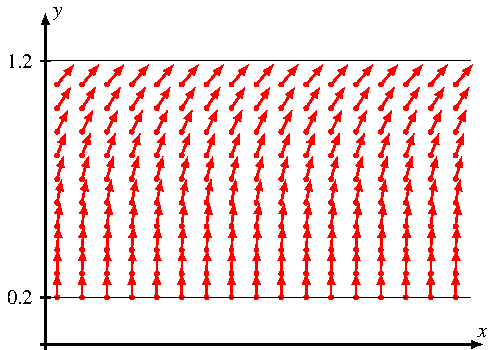
\includegraphics[width=0.48\hsize]{chapters/2/upright.pdf}
\hspace{0.02\hsize}
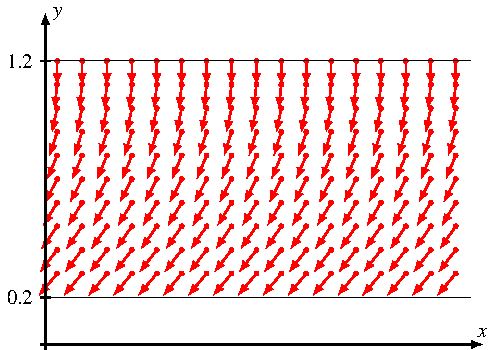
\includegraphics[width=0.48\hsize]{chapters/2/downright.pdf}
\caption{Simulation der Strömung in gemässigten Breiten der Nordhalbkugel
mit Hilfe des Modells
\eqref{section:coriolis:udgl}
und
\eqref{section:coriolis:vdgl}.
Die Strömung wird unter dem Einfluss der Coriolis-Beschleunigung nach
rechts abgelenkt ($\beta=1.2$, $h=0.1$).
\label{section:coriolis:simbild}}
\end{figure}
Wie schon angedeutet kann man nicht davon ausgehen, eine analytische
Lösung des Differentialgleichungssystems~\eqref{skript:coriolis:udgl}
und \eqref{skript:coriolis:vdgl}
finden zu können.
Wir beschränken uns daher auf eine numerische Lösung und lösen
lösen das Systems mit Hilfe von Octave mit der Implementation
\lstinputlisting[style=Matlab]{chapters/2/coriolisdgl.m}
der Differentialgleichung.
Als Anfangswerte wurde einerseits eine von $y_0=0.2$ ausgehende nordwärts
gerichtete Strömung bis $y=1.2$ simuliert und andererseits eine südwärts
gerichtete Strömung von $y_0=1.2$ bis $y=0.2$
(Abbildung~\ref{section:coriolis:simbild}).
Es wurden die Parameter $\beta=1.2$ und $h=-0.1$ verwendet.
In beiden Fällen kann die Rechtsablenkung durch die Coriolisbeschleunigung
beobachtet werden.

In der Simulation zu den Abbildungen
\ref{skript:stream-graph}
und
\ref{skript:cross-graph}
wurde bereits bemerkt, dass ein einzelnes Teilchen auf der Erdoberfläche
der Rechtsablenkung durch die Coriolis-Kraft ausgesetzt ist,
jedoch ergaben sich für eine Strömung nicht realistische Bahnen.
Das vorliegende Strömungsdynamische Modell zeigt dagegen, wie
realistische Stromlinien aussehen müssen.

Die Simulationen zeigen auch, dass die $u$-Komponente stark anwächst,
und zwar umso schneller, je grösser der Faktor $\beta$ ist.
Man kann dies als Indiz dafür deuten, dass die Strömung nicht beliebig
lange nach Norden oder Süden fliessen kann, dass sich also zonale
Strömungen mit alternierenden Druckgradienten ausbilden werden, wie man
sie auf dem Jupiter (Abbildung~\ref{skript:jupiterzirkulation} oder
in der globalen Zirkulation der Erde wie in
Abbildung~\ref{skript:globalezirkulation} dargestellt beobachtet.


